\documentclass[14pt,a4paper,report]{report}
\usepackage[a4paper, mag=1000, left=2.5cm, right=1cm, top=2cm, bottom=2cm, headsep=0.7cm, footskip=1cm]{geometry}
\usepackage[utf8]{inputenc}
\usepackage[english,russian]{babel}
\usepackage{indentfirst}
\usepackage[dvipsnames]{xcolor}
\usepackage[colorlinks]{hyperref}
\usepackage{listings} 
\usepackage{fancyhdr}
\usepackage{caption}
\usepackage{amsmath}
\usepackage{latexsym}
\usepackage{graphicx}
\usepackage{amsmath}
\hypersetup{
	colorlinks = true,
	linkcolor  = black
}

\usepackage{titlesec}
\titleformat{\chapter}
{\Large\bfseries} % format
{}                % label
{0pt}             % sep
{\huge}           % before-code


\DeclareCaptionFont{white}{\color{white}} 

% Listing description
\usepackage{listings} 
\DeclareCaptionFormat{listing}{\colorbox{gray}{\parbox{\textwidth}{#1#2#3}}}
\captionsetup[lstlisting]{format=listing,labelfont=white,textfont=white}
\lstset{ 
	% Listing settings
	inputencoding = utf8,			
	extendedchars = \true, 
	keepspaces = true, 			  	 % Поддержка кириллицы и пробелов в комментариях
	language = Matlab,            	 	 % Язык программирования (для подсветки)
	basicstyle = \small\sffamily, 	 % Размер и начертание шрифта для подсветки кода
	numbers = left,               	 % Где поставить нумерацию строк (слева\справа)
	numberstyle = \tiny,          	 % Размер шрифта для номеров строк
	stepnumber = 1,               	 % Размер шага между двумя номерами строк
	numbersep = 5pt,              	 % Как далеко отстоят номера строк от подсвечиваемого кода
	backgroundcolor = \color{white}, % Цвет фона подсветки - используем \usepackage{color}
	showspaces = false,           	 % Показывать или нет пробелы специальными отступами
	showstringspaces = false,    	 % Показывать или нет пробелы в строках
	showtabs = false,           	 % Показывать или нет табуляцию в строках
	frame = single,              	 % Рисовать рамку вокруг кода
	tabsize = 2,                  	 % Размер табуляции по умолчанию равен 2 пробелам
	captionpos = t,             	 % Позиция заголовка вверху [t] или внизу [b] 
	breaklines = true,           	 % Автоматически переносить строки (да\нет)
	breakatwhitespace = false,   	 % Переносить строки только если есть пробел
	escapeinside = {\%*}{*)}      	 % Если нужно добавить комментарии в коде
}

\begin{document}

\def\contentsname{Содержание}

% Titlepage
\begin{titlepage}
	\begin{center}
		\textsc{Санкт-Петербургский Политехнический 
			Университет Петра Великого\\[5mm]
			Кафедра компьютерных систем и программных технологий}
		
		\vfill
		
		\textbf{Отчёт по лабораторной работе №2\\[3mm]
			Курс: «Теория автоматического управления»\\[3mm]
			}
	\end{center}
	
	\hfill
	\begin{minipage}{.5\textwidth}
		Выполнил студент:\\[2mm] 
		Балсутьев Владимир\\
		Группа: 43501/4\\[5mm]
		
		Проверил:\\[2mm] 
		Нестеров Сергей Александрович
	\end{minipage}
	\vfill
	\begin{center}
		Санкт-Петербург\\ \the\year\ г.
	\end{center}
\end{titlepage}

% Contents
\tableofcontents
\clearpage

\chapter{Лабораторная работа №2}

\section{Цель работы}

Получить навыки работы с моделями ВСВ и каноническими представлениями.

\section{Программа работы}

\begin{itemize}
	\item Представить систему в трех канонических формах.
	\item Получить структурные схемы для каждой формы.
\end{itemize}

\section{Индивидуальное задание}

$
\\
y''+ y=u, y(0)=0, y'(0)=0,y''(0)=0, u=1(t)\\\\
W(p)=\frac{y}{u}=\frac{1}{p^2+1}
$

\section{Ход работы}

\subsection{Построение канонических форм}

\subsubsection{Нормальная форма управления}

\begin{equation*}
\text{$W(p)=\frac{1}{p^2+1}=\frac{y}{u}$}
\end{equation*}

\begin{equation*}
\text{$\frac{y}{1}=\frac{u}{p^2+1}=x_1$}
\Longrightarrow
\begin{cases}
	\text{$u=x_1(p^2+1)$} \\
	\text{$y=x_1(1)$}
\end{cases}
\end{equation*}

\begin{equation*}
\begin{cases}
	\text{$px_1=x_2$} \\
	\text{$px_2=u-x_1$}\\
	\text{$y=x_1$}
\end{cases}
\end{equation*}

\begin{equation*}
\text{$A=$}
\text{$
\begin{bmatrix}
0 & 1 \\
-1 & 0 \\
\end{bmatrix}
$}
\text{$, B=$}
\text{$
\begin{bmatrix}
0 \\
1 \\
\end{bmatrix}
$}
\text{$, C=$}
\text{$
\begin{bmatrix}
1 & 0 \\
\end{bmatrix}
$}
\end{equation*}

Проверим корректность полученных матриц $A, B, C$:

\begin{equation*}
\text{$det(A-\lambda)=0$}
\Longrightarrow
\text{$ \lambda^2 + 1=0$}
\Longrightarrow
\begin{cases}
	\text{$\lambda_1=i$} \\
	\text{$\lambda_2=-i$}
\end{cases}
\end{equation*}

Собственные числа совпадают с собственными числами матриц в нормальной форме наблюдения и канонической форме, что свидетельствует о корректности полученных матриц  $A, B, C$.

\begin{equation*}
\text{$W(p)=C(pE-A)^{-1}B=
\begin{bmatrix}
1 & 0\\
\end{bmatrix}
\begin{bmatrix}
p & -1 \\
1 & p\\
\end{bmatrix}^{-1}
\begin{bmatrix}
0 \\
1 \\
\end{bmatrix}=
\frac{1}{p^2 + 1}
\begin{bmatrix}
1 & 0 \\
\end{bmatrix}
\begin{bmatrix}
p & 1 \\
-1 & p\\
\end{bmatrix}
\begin{bmatrix}
0 \\
1 \\
\end{bmatrix}
\Longrightarrow
$}
\end{equation*}

\begin{equation*}
\text{$ W(p) = \frac{1}{p^2 + 1}$} 
\end{equation*}

Передаточная функция, полученная в результате преобразования $W(p)=C(pE-A)^{-1}B$, полностью совпадает с исходной, что свидетельствует о корректности полученных матриц  $A, B, C$. 

%\begin{figure}[h!]
%	\centering
%	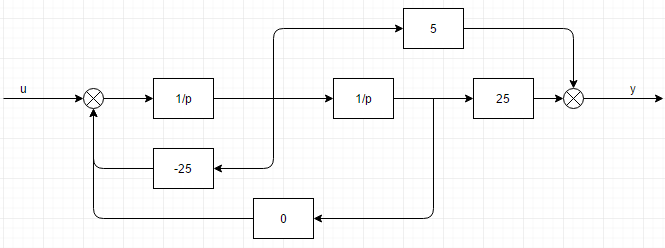
\includegraphics[scale = 0.73]{images/nfu.png}
%	\caption{Структурная схема НФУ}
%	\label{image:1}
%\end{figure}

\subsubsection{Нормальная форма наблюдения}

\begin{equation*}
\text{$W(p)=\frac{1}{p^2 + 1}=\frac{y}{u}$}
\Longrightarrow
\text{$u=(p^2 + 1)y$}
\Longrightarrow
\end{equation*}

\begin{equation*}
\Longrightarrow
\text{$y(p^2 +1)- u=0$}
\Longrightarrow
\text{$p(p(y)) + y - u =0$}
\end{equation*}

\begin{equation*}
\begin{cases}
	\text{$x_1=py$} \\
	\text{$px_1= u - y$} \\
\end{cases}
\Longrightarrow
\begin{cases}
	\text{$x_2=y$}\\
	\text{$x_1=px_2$} \\
	\text{$px_1=u - x_2$} \\
\end{cases}
%\Longrightarrow
%\begin{cases}
%	\text{$px_1=25u$} \\
%	\text{$px_2=x_1-25x_2+5u$} \\
%	\text{$y=x_2$}
%\end{cases}
\end{equation*}

\begin{equation*}
\text{$A=$}
\text{$
	\begin{bmatrix}
	0 & -1 \\
	1 & 0 \\
	\end{bmatrix}
	$}
\text{$, B=$}
\text{$
	\begin{bmatrix}
	1 \\
	0 \\
	\end{bmatrix}
	$}
\text{$, C=$}
\text{$
	\begin{bmatrix}
	0 & 1 \\
	\end{bmatrix}
	$}
\end{equation*}

Проверим корректность полученных матриц $A, B, C$:

\begin{equation*}
\text{$det(A-\lambda)=0$}
\Longrightarrow
\text{$ (-\lambda^2) - (-1) * 1=0$}
\Longrightarrow
\begin{cases}
	\text{$\lambda_1=i$} \\
	\text{$\lambda_2=-i$}
\end{cases}
\end{equation*}

Собственные числа совпадают с собственными числами матриц в нормальной форме управления и канонической форме, что свидетельствует о корректности полученных матриц  $A, B, C$.

\begin{equation*}
\text{$W(p)=C(pE-A)^{-1}B=
\begin{bmatrix}
0 & 1 \\
\end{bmatrix}
\begin{bmatrix}
p & 1 \\
-1 & p\\
\end{bmatrix}^{-1}
\begin{bmatrix}
1 \\
0 \\
\end{bmatrix}=
\frac{1}{p^2 + 1}
\begin{bmatrix}
0 & 1 \\
\end{bmatrix}
\begin{bmatrix}
p & -1 \\
1 & p \\
\end{bmatrix}
\begin{bmatrix}
1 \\
0 \\
\end{bmatrix}
$}
\Longrightarrow
\end{equation*}

\begin{equation*}
\text{$
W(p) = \frac{1}{p^2+1}
$}
\end{equation*}

Передаточная функция, полученная в результате преобразования $W(p)=C(pE-A)^{-1}B$, полностью совпадает с исходной, что свидетельствует о корректности полученных матриц  $A, B, C$. 

\clearpage

%\begin{figure}[h!]
%	\centering
%	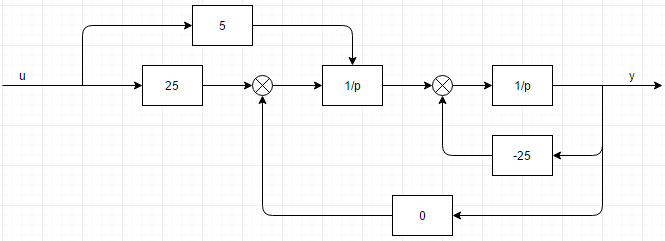
\includegraphics[scale = 0.67]{images/nfn.png}
%	\caption{Структурная схема НФН}
%	\label{image:2}
%\end{figure}

\subsubsection{Каноническая форма}

\begin{equation*}
\text{$W(p)=\frac{1}{p^2 + 1}=\frac{1}{(p + i)(p - i)}=\frac{-0.5i}{p - i} + \frac{0.5i}{p + i} = \frac{y}{u}$}
\end{equation*}

\begin{equation*}
\begin{cases}
	\text{$\frac{x_1}{u}=\frac{-0.5i}{p - i}$} \\
	\text{$\frac{x_2}{u}=\frac{0.5i}{p + i}$} \\
	\text{$y = x_1 + x_2$}
\end{cases}
\Longrightarrow
\begin{cases}
\text{$px_1= - \frac{1}{2} i u + i*x_1$} \\
\text{$px_2= \frac{1}{2} i u - i*x_2$} \\
\text{$y=x_1+x_2$}
\end{cases}
\end{equation*}

\begin{equation*}
\text{$A=$}
\text{$
	\begin{bmatrix}
	i & 0 \\
	0 & -i \\
	\end{bmatrix}
	$}
\text{$, B=$}
\text{$
	\begin{bmatrix}
	-\frac{1}{2}i \\
	 \frac{1}{2}i \\
	\end{bmatrix}
	$}
\text{$, C=$}
\text{$
	\begin{bmatrix}
	1 & 1 \\
	\end{bmatrix}
	$}
\end{equation*}

Проверим корректность полученных матриц $A, B, C$:

\begin{equation*}
\text{$det(A-\lambda)=0$}
\Longrightarrow
	\text{$(\lambda - i)(\lambda + i)=0$}
\Longrightarrow
\begin{cases}
	\text{$\lambda_1=i$} \\
	\text{$\lambda_2=-i$}
\end{cases}
\end{equation*}

Собственные числа совпадают с собственными числами матриц в нормальной форме управления и нормальной форме наблюдения, что свидетельствует о корректности полученных матриц  $A, B, C$

\begin{equation*}
\text{$W(p)=C(pE-A)^{-1}B=
	\begin{bmatrix}
	1 & 1 \\
	\end{bmatrix}
	\begin{bmatrix}
	i & 0 \\
	0 & -i\\
	\end{bmatrix}^{-1}
	\begin{bmatrix}
	-\frac{1}{2}i \\
	 \frac{1}{2}i \\
	\end{bmatrix}=
	\begin{bmatrix}
	1 & 1 \\
	\end{bmatrix}
	\begin{bmatrix}
	\frac{1}{p - i} & 0 \\
	0 & \frac{1}{p + i}
	\end{bmatrix}
	\begin{bmatrix}
	-\frac{1}{2}i \\
	 \frac{1}{2}i \\	\end{bmatrix}=
	$}
\end{equation*}

\begin{equation*}
\text{$=\begin{bmatrix}
	\frac{1}{p - i} & \frac{1}{p + i} \\
	\end{bmatrix}\begin{bmatrix}
	-\frac{1}{2}i \\
	 \frac{1}{2}i \\	
	 \end{bmatrix}= -\frac{0.5i}{p - i} + \frac{0.5i}{p + i}
	$}
\end{equation*}

Передаточная функция, полученная в результате преобразования $W(p)=C(pE-A)^{-1}B$, полностью совпадает с исходной, что свидетельствует о корректности полученных матриц  $A, B, C$. 


%\begin{figure}[h!]
%	\centering
%	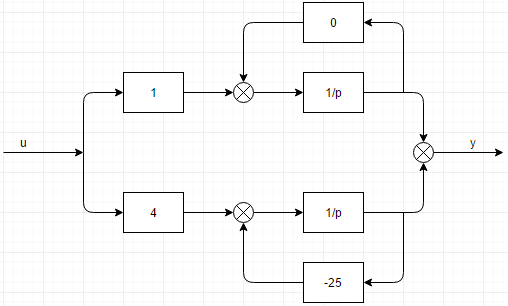
\includegraphics[scale = 0.67]{images/kf.png}
%	\caption{Структурная схема КФ}
%	\label{image:3}
%\end{figure}


\section{Вывод}

Модель ВСВ весьма гибкая, так как помимо трех канонических форм, рассмотренных в работе существуют произвольные формы, которые иногда могут быть полезны. 

Отличия между каноническими формами наиболее явно проявляются на структурных схемах. Система, представленная в форме управления, имеет два узла суммирования и n узлов размножения. В форме наблюдения - наоборот, два узла размножения и n узлов суммирования. Особенность обеих этих форм - сложные обратные связи между элементами схемы.


\end{document}\textsl{•}